\documentclass[8pt]{article}
\usepackage{url}
\usepackage{graphicx}
\usepackage{amsmath}
\usepackage{caption}
\usepackage{subcaption}
\begin{document}
\pagestyle{empty}
\title{\huge{ECE~741 Wireless Networks\\Term Paper\\Spring, 2017}
\vspace{50mm} \\\LARGE{\emph{Performance and efficiency analysis of DRX (Discontinuous Reception) power saving in 3GPP LTE}}\vspace{50mm}
\\\large{Alem Abreha\\ G00741281}\vspace{5mm}
\\\large{George Mason University\\Fairfax, VA}}
\date{}
\maketitle
%%%%%%%%%%%%%%%%%%%%%%%%%%%%%%%%%%%%%%%%%%%%%%%%%%%%%%%%%%%%%%%%%%%%%
\section*{Abstract}

Discontinuous Reception (DRX) is one way of saving power for many forms of mobile wireless devices that depend on battery for power source. DRX offers power saving opportunity by turning off radio transceiver during inactive periods at the cost of incurring transmission delay time. The power saving factor gained can be an indicator of performance for DRX operation, while the wake-up delay can be interpreted as indicator of DRX efficiency. These two parameters are used to numerically measure the performance and efficiency of DRX by taking a simplified or semi-markov analytical models.
 

\section*{Introduction}

 The 3GPP (Third Generation Partnership Project) collaboration is continually ramping up the specification of LTE/LTE-Advanced (referred to as LTE generally) in terms of bitrate(bandwith) and latency. The evolution in storage, processing power, RF transceivers and battery technology are the underlying enablers that are  allowing the continuously increasing capacity of LTE networks\cite{holma2012lte}. The demand for higher bandwidth and lower latency by users and applications is also growing in parallel. 

%\vspace{5mm} 

\begin{figure}[h!]
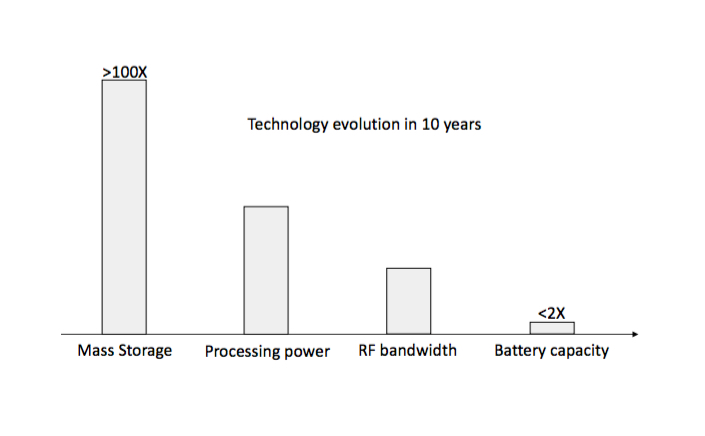
\includegraphics[width=\linewidth]{technology_evolution_by_alem.png}
\caption{Evolution of underlying components enabling LTE technology}
\label{fig:evolution}
\end{figure}

This growing demand of users and applications is accompanied by high battery consumption on the UE (User Equipment) side due to more signaling and IO (input output) processing. On the contrary, battery technology has not seen any sizable advancement as compared to the other technological components Figure 1 \cite{holma2012lte}. Energy density in batteries has remained the same during the 3G to LTE advancement. Because of this reason UE power consumption remains a challenge and substantial improvements in energy-efficient mechanisms will continue to be fundamental for operating the very high bit rates in LTE \cite{6363708}. LTE implements DRX power saving mechanism during both connected (RRC\_CONNECTED) and idle (RRC\_IDLE) states.

\subsection*{DRX cycle description}
The key idea behind DRX is saving UE power consumption by turning off the radio transceiver (sleep) during periods when there are no packets incoming from the evolved node base station (eNodeB), and then by monitoring the physical downlink control channel (PDCCH) for indication message of incoming packets to make the decision of turning on the transceiver (wakeup).   

\begin{figure}[h!]
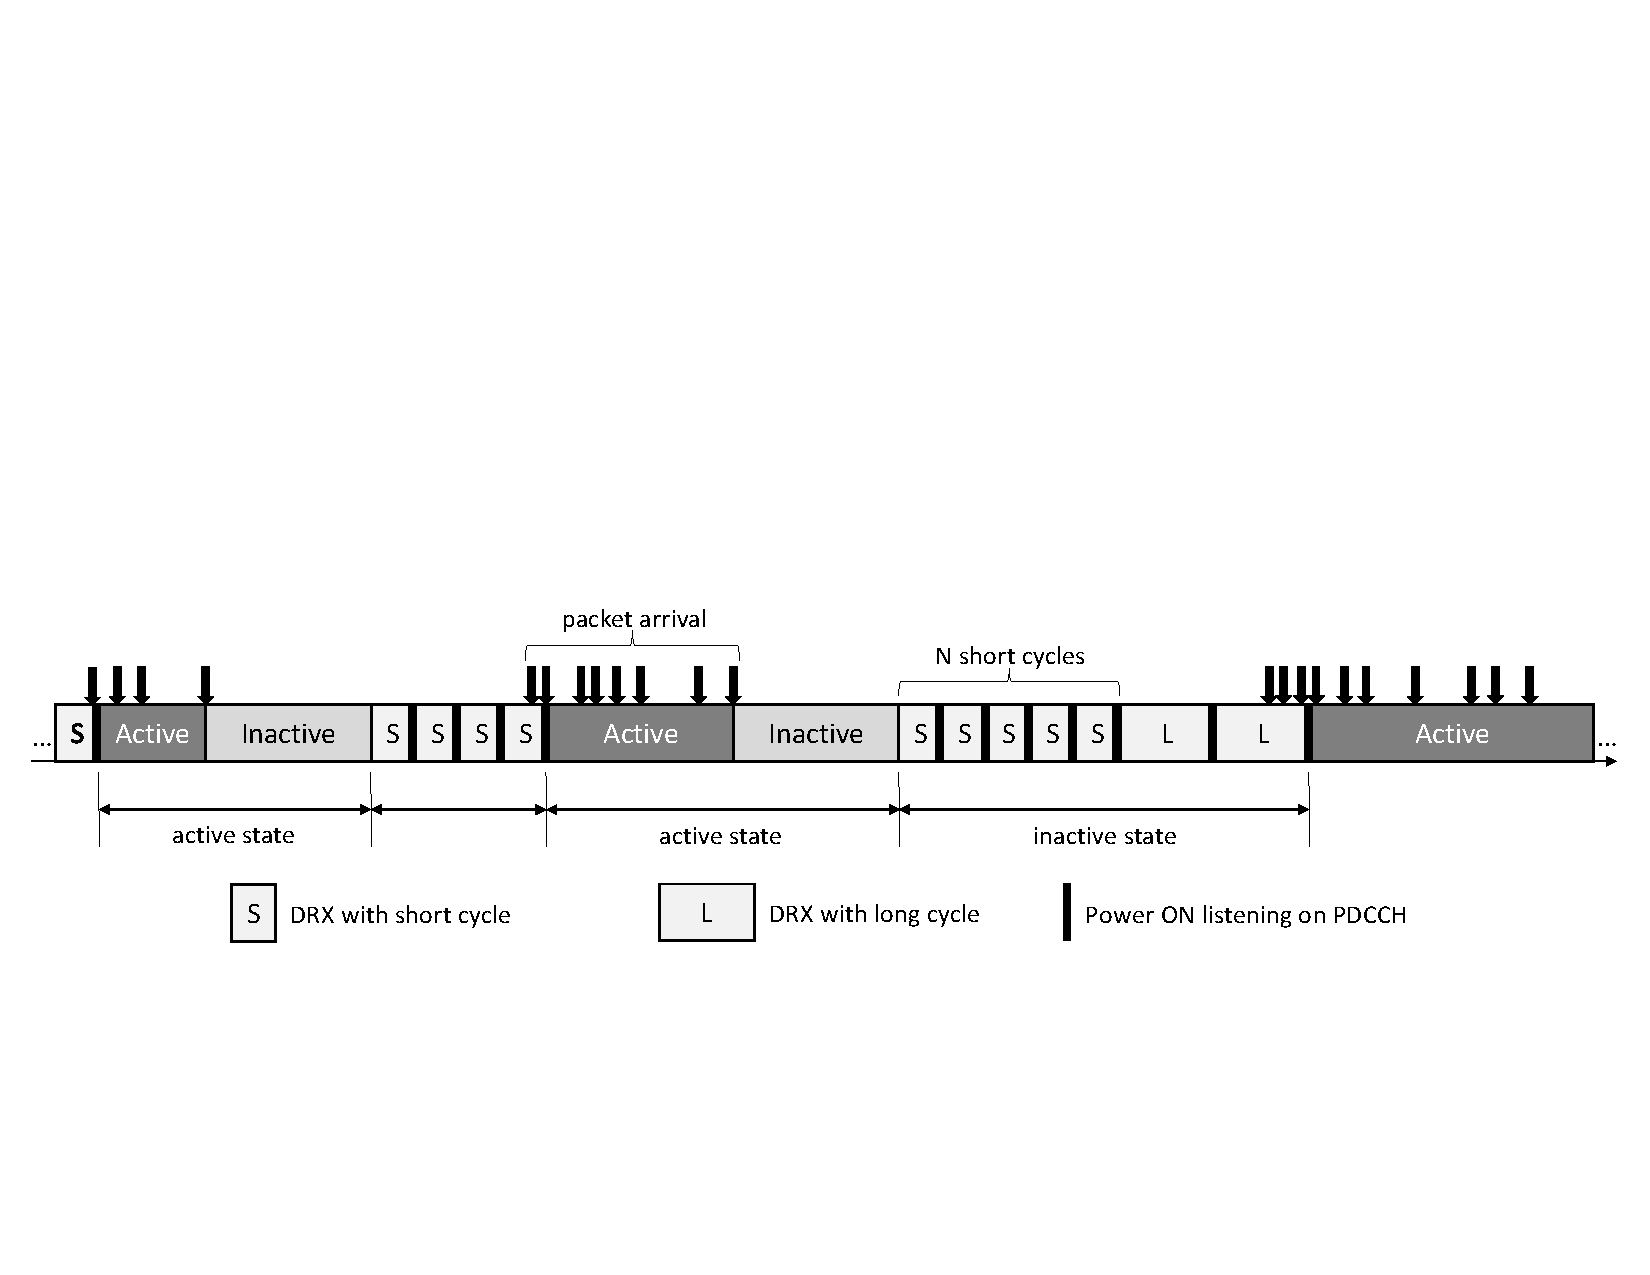
\includegraphics[width=\linewidth]{drx_cycle_alem.png}
\caption{DRX Operation} 
\label{fig:DRX}
\end{figure}
The detailed operation of DRX follows the illustration in Figure 2. A DRX cycle is a time duration that the UE goes into a sleep period followed by waking up temporarily to receive indication messages through the PDCCH channel. When the UE receives a negative indication message, it goes back to sleeping period. On the other hand, upon reception of a positive indication message, the UE stays awake to receive buffered packets. Packets that are transmitted to the UE while the UE is in DRX sleep cycles will get buffered until the UE comes out of a DRX cycle.
 
 
DRX cycles are denoted by rectangles, with letters "S" and "L" standing for short and long DRX cycles, respectively. When UE enters into DRX after the inactivity timer \(t_I\) expired, it goes into DRX short cycles and monitoring PDCCH at the end of each short cycle. When enough number of DRX short cycles (N) take place without detection of incoming packets, the DRX short cycle timer \(t_N\) expires. Following the UE will start entering DRX long cycles, sleeping for longer periods and waking up temporarily to check the PDCCH channel for incoming packets at the end of each long cycle. 


DRX operation is confined by the following four configuration parameters:\newline
1. \(t_{DS}\) : DRX short cycle duration\newline
2. \(t_{DL}\) : DRX long cycle duration\newline
3. \(t_{I}\) : DRX inactivity timer\newline
4. \(t_{N}\) : DRX short cycle timer\newline

DRX Short and Long Cycles specify the periodic repetition of On duration, which is of fixed value applied to both cycles. During On duration, UE monitors the PDCCH to see if there is any transmission over the shared data channel destined to this UE. DRX inactivity timer defines the period during which UE shall stay awake monitoring PDCCH after the last successful decoding of PDCCH before entering DRX operation. DRX short cycle timer specifies the period during which UE shall follow DRX short cycle after DRX inactivity timer has expired. UE enters DRX long cycle periods if the DRX short cycle timer expired and there is no positive indication of buffered packets on PDCCH \cite{4657144}.

DRX offers power saving opportunity at the cost of and wake up delay time, hence power saving factor \(PS\) can be an indicator of performance, while the wake-up delay \(D\) can be interpreted as indicator of efficiency. PS is the percentage of time UE spends in sleeping. D is the average waiting time a packet call delivery experiences before UE wakes up. Hence, PS and D are used to numerically measure the performance and efficiency of DRX configurations.

\section*{Problem and Approach}
\subsection*{Simplified Analytical Model}

\cite{6151867} developed a simplified model by breaking down the DRX operation into several independent parts and then combined the result obtained in each part to compute PS and D. In this model, indication message transmission time is assumed to be very short and hence neglected in the analysis. Packet service time is also assumed to be larger than the inter-packet arrival time, and UE enters the power saving mode only after the service of a whole packet call.

PS is expressed as the ratio the time spent sleeping to the overall operation.\newline

\begin{equation}
	PS = E[T_{D}]/\left(E[T_{A}] + E[T_{D}]\right)
\end{equation}

E[\(T_{D}\)] and E[\(T_{A}\)] are derived into the following closed-form equations as shown in \cite{6151867} :

\begin{equation}
 E[T_{D}]= {\hbox{1} - (e^{-\lambda t_{DS}})^{N} \over \hbox{1} - e^{-\lambda t_{DS}}} t_{DS} + {(e^{-\lambda t_{DS}})^{N}\over \hbox{1} - e^{-\lambda t_{DL}}} t_{DL}		
\end{equation}

\begin{equation}
 E[T_{A}] = {\rho\over \hbox{1} - \rho} E[T_{D}] + {\hbox{1}\over \lambda (\hbox{1} - \rho)} (e^{\lambda t_{I}} - \hbox{1})
\end{equation}

Where N is the number of DRX short cycles before \(t_{N}\) expires and the first DRX long cycle period starts. \(\rho\) is the traffic intensity of the exponential packet interval with expectation 1/\(\lambda\). \(\tau\) is the expectation of packet transmission time (processing time).
\begin{equation}
	\rho = \lambda\tau
\end{equation}
Substituting equations (2) and (3) in (1), PS is expressed using the following equation as a function of \(\rho\), \(\lambda\), N, \(t_{DS}\), \(t_{DL}\) and \(t_{I}\)

\begin{equation}
	(\hbox{1} - \rho) \times \left({\hbox{1} - (e^{- \lambda t_{DS}})^{N}\over \hbox{1} - e^{-\lambda t_{DS}}} t_{DS} + {(e^{-\lambda t_{DS}})^{N}\over \hbox{1} - e^{- \lambda t_{DL}}}t_{DL} \right) \over \left({\hbox{1} \!-\! (e^{-\lambda t_{DS}})^{N}\over \hbox{1} \!-\! e^{-\lambda t_{DS}}} t_{DS} \!+\! {(e^{-\lambda t_{DS}})^{N}\over \hbox{1} \!-\! e^{-\lambda t_{DL}}}t_{DL} \!+\! {\hbox{1}\over \lambda} (e^{\lambda t_{I}} \!-\! \hbox{1})\right)
\end{equation}

In order to analyze the transmission delay D, DRX is broken into two states : intermediate-transmitting state with \(E[D_{I}]\) and buffering-and-forwarding state with \(E[D_{BS}]\) or \(E[D_{BL}]\). \(E[D_{BS}]\) and \(E[D_{BL}]\) are expected transmission delays in buffering-and-forwarding state for DRX short and long cycle periods respectively. Considering these two states average transmission delay \(E[D]\) can be generally expressed as follows.
\begin{equation}
	E[D] = P_{on}*E[D_I] + P_{DS}*(E[D_{I}] + E[D_{BS}]) + P_{LS}*(E[D_{I}] + E[D_{BL}])
\end{equation}
Where \(P_{on}\) = Probability of UE receiver power ON, \(P_{DS}\) = Probability of UE in DRX short cycle and \(P_{LS}\) = Probability of UE in DRX long cycle.

%	The immediate-transmitting state is treated as M/G/1 queuing model because, newly arrived packet is immediately accepted if the Radio Network Controller (RNC) buffer is empty or it might get delayed if the buffer is not empty and other packets are already in queue. The average packet transmission delay \(E[D_{I}]\) is expressed as follows, using Pollaczek-Khinchine formula \cite{takagi1991queueing}. 
%
%\begin{equation}
%	E[D_{I}] = {\lambda E[X^{2}]\over \hbox{2} (\hbox{1} - \rho)}
%\end{equation}

%The second order moment of the exponential random variable X is given by 
%
%\begin{equation}
%	E[X^{2}] = {\hbox{2}\over \lambda^2}. 
%\end{equation}
% 
% In buffering-and-forwarding state packets experience a delay that is a combination of delay due to the buffering operation as in (6) \(E[W]\)and due to packets that are already in the buffer. The later is a product of average transmission time \(E[X]\) and average number of packets waiting in buffer. Hence the delay due to buffering is given by
% 
% \begin{equation}
% 	E[D_{B}] = E[W] + E[X]E[K].
% \end{equation} 
%
%But from Little's law we have,
%\begin{equation}
%	E[D_{B}] = {{1\over\lambda}E[K]}.
%\end{equation}
%
%Combining (8) and (9)
%
%\begin{equation}
%	E[D_{B}] = {E[W]\over \hbox{1} - \rho}
%\end{equation}
%
%Overall average packet delay is the sum of the transmission delay \(D_{I}\) and buffering delay \(D_{B}\) while accounting for the probability of UE being in power active (1 - \(P_{S}\) - \(P_{L}\)), DRX short cycle (\(P_{S}\)) and DRX long cycle (\(P_{L}\)). Expressed as,
%
%\begin{equation}
%	E[D] = (\hbox{1} \!-\! P_{S} \!-\! P_{L}) E[D_{I}] \!+\! P_{S} \left(E[D_{I}] \!+\! (E[D_{BS}]) \right) \!+\! P_{L} \left(E[D_{I}] \!+\! (E[D_{BL}]) \right).
%\end{equation}
%
%Where \(E[D_{BS}]\) and \(E[D_{BL}]\) are average waiting times in buffering incurred due to DRX short and long cycles respectively and expressed in the same format as (10). 
%\begin{equation}
%	E[D_{BS}] = {E[t_{S}]\over \hbox{1} - \rho} , \  E[D_{BL}] = {E[t_{L}]\over \hbox{1} - \rho} 
%\end{equation}
%According to the property of the Poisson process, packet arrival time instants are uniformly distributed in a given time period, \(t_{DS}\) or \(t_{DL}\) in DRX. For uniform distribution,
%
%\begin{equation}
%	E[t_{S}] = {t_{DS}\over \hbox{2}} , \  E[t_{L}] = { t_{DL} \over \hbox{2} }
%\end{equation} 
%
%\(P_{S}\) and \(P_{L}\) are given by,
%\begin{equation}
%	P_{S} = {E[t_{S}]\over \left(E[T_{A}] + E[T_{D}] \right)} , \  
%	P_{L} = {E[t_{L}]\over \left(E[T_{A}] + E[T_{D}] \right)}.
%\end{equation}
%
%By combining (6),(7),(11),(12),(13) and (14) average packet delay is expressed as a function of \(\rho\), \(\lambda\), N, \(t_{DS}\), \(t_{DL}\) and \(t_{I}\) as shown in (15).

The general expression of D in (6) is reduced into the closed form expression in (7) \cite{6151867}. 
\begin{equation}
\begin{aligned}
E[D] = {\hbox{1}\over \lambda (\hbox{1} \!-\! \rho)}\ + \\
&   {\hbox{1}\over \hbox{2}} \left({\hbox{1} \!-\! (e^{-\lambda t_{DS}})^{N}\over \hbox{1} \!-\! e^{-\lambda t_{DS}}} (t_{DS})^{2} \!+\! {(e^{-\lambda t_{DS}})^{N}\over \hbox{1} \!-\! e^{-\lambda t_{DL}}} (t_{DL})^{2} \right) \bigg/ \cr&\left({\hbox{1} \!-\! (e^{-\lambda t_{DS}})^{N} \over \hbox{1} \!-\! e^{-\lambda t_{DS}}} t_{DS} \!+\! {(e^{-\lambda t_{DS}})^{N}\over \hbox{1} \!-\! e^{-\lambda t_{DL}}}t_{DL} \!+\! {\hbox{1}\over \lambda} (e^{\lambda t_{I}} \!-\! \hbox{1}) \right)
\end{aligned}
\end{equation}

\subsection*{Semi-Markov Chain Analytical Model}

\cite{6363708}, \cite{1690890893}, \cite{7303883} and \cite{6654993} took a semi-markov model approach to analyze the performance and efficiency of DRX operation. \cite{6363708} and \cite{1690890893} have further advanced the analysis respectively by making the length of DRX short and long cycles adjustable. In the case of adjustable DRX for contiguous sleep cycles, the duration of the \(n^{th}\) sleep interval is obtained by :
\begin{equation*}
T(n)=\begin{cases} 
		\kappa 2^{n} & 1\leq {n}<{M}
		\\ 
		T_{\max} & {M}\leq {n}
	\end{cases}
\end{equation*}
where M is the value that T(n)=\(T_{max}\) and \(\kappa\) is a rescaling factor, which is used to control the total sleep cycle duration in both cases of \cite{6363708} and \cite{1690890893}. The semi-markov analysis of DRX opreration is represented by the state transition diagram as shown in Figure 3.
\\
State 1 (S1) : comprises sequence of adjacent active time intervals where the UE power is ON.
\\
State 2 (S2) : represents periods during which UE follows DRX short cycles.
\\
State 3 (3) :  represents periods during which UE follows DRX long cycles.
\begin{figure}[h!]
\includegraphics[width=1\linewidth]{semi-markov.png}
\caption{A semi-markov process for DRX operation analysis} 
\label{fig:DRX}
\end{figure}

The transition probability matrix and the balance equations are solved as follows for the Markov process explained above \cite{6363708}.
\begin{equation}
	{P}= \begin{bmatrix} 
				P11 & P12 & 0 \\ 
	            P21 & 0 & P23 \\ 
	            1 & 0 & 0
	     \end{bmatrix}
\end{equation}
\begin{equation}
	\prod=\begin{cases} \pi_{1}\ =\ {1 \over 1+P11+P12*P23}\cr \pi_{2}\ =\ {P12 \over 1+P12+P12*P23}\cr \pi_{3}\ =\ {P12*P23\over 1+P12+P12*P23} 
          \end{cases}	
\end{equation}

Equations (8) and (9)  used to derive closed form expressions for 	PS and D in \cite{6363708} and \cite{1690890893} in similar procedures. \cite{6363708} made the DRX short cycles adjustable while \cite{1690890893} did the same for DRX long cycles. Both resulted in a slight PS gain as compared to fixed cycles at the cost of higher transmission delay, but in this paper the discussion considers only fixed duration DRX cycles.

PS is equal to the probability that the semi-Markov process is at S2 and S3 in the steady state.
\begin{equation}
	PS={\pi_{2}E\left[S_{2}\right]+\pi_{3}E\left[S_{3}\right]\over \sum\nolimits_{i=1}^{3}\pi_{i}E[S_{i}]}
\end{equation}

Similarly D is the expected time that the UE resides in DRX short and long sleep cycles, which can be expressed as follows :
\begin{equation}
	E[D]=\sum_{i=1}^{N}p_{i}{t_{DS}\over 2}+\sum_{i=N+1}^{\infty}p_{i}{t_{DL}\over 2}
\end{equation} 

Where \(p_{i}\) is the probability that the packet delivery starts during the \(i^{th}\) DRX cycle is given by :
\begin{equation}
	p_{i}=\begin{cases} P_{pc}e^{-\lambda _{ipc}t_{I}}e^{-\lambda _{ipc}(i-1)t_{DS}}(1-e^{-\lambda _{ipc}t_{DS}})\cr \underbrace{+P_{s}e^{-\lambda _{is}t_{I}}e^{-\lambda _{is}(i-1)t_{DS}}(1-e^{-\lambda _{is}{t_{DS}}})}_{1\leq i\leq N}\cr P_{pc}e^{-\lambda _{ipc}[(t_{I}+Nt_{DS}+(i-N-1)t_{DL}]}(1-e^{-\lambda _{ipc}{t_{DL}}})\cr +\underbrace{ P_{s}e^{-\lambda _{is}[(t_{I}+Nt_{DS}+(i-N-1)t_{DL}]}(1-e^{-\lambda _{is}{t_{DL}}})}_{i\geq N}	
\end{cases}
\end{equation} 
Where \(\lambda _{ipc}\) , \(P_{pc}\) , \(\lambda _{is}\) and \(P_{s}\) are the arrival rate and probability for single packet call and session respectively.
\section*{Simulation and Results}

Taking simulation parameters \(\rho\) = 0.01, \(\lambda\) = 0.1, N = 2 and \(t_{DL}\) = 2 x \(t_{DS}\). Figure 4 shows the effects of varying \(t_{I}\) on PS and delay. As \(t_{DS}\) increases the UE will be be residing in longer DRX short cycles which results in higher PS but with the penalty of delay. Having higher \(t_{I}\) favors delay since UE will be waiting longer in power active mode.

\begin{figure}[h!]
\centering
\begin{subfigure}{.5\textwidth}
  \centering
  \includegraphics[width=1\linewidth]{ps_model_1_tI.png}
  \caption{ PS vs \(t_{DS}\)}
  \label{fig:sub1}
\end{subfigure}%
\begin{subfigure}{.5\textwidth}
  \centering
  \includegraphics[width=1\linewidth]{delay_model_1_tI.png}
  \caption{Delay vs \(t_{DS}\)}
  \label{fig:sub2}
\end{subfigure}
\caption{PS and Delay vs \(t_{DS}\) for different settings of  \(t_{I}\)}
\label{fig:test}
\end{figure}


Figure 5 shows the implication of \(t_{DL}\) on PS and Delay as a function of N (number of DRX short cycles before entering DRX long cycles) while keeping \(t_{DS}\)=10msec.

\newpage

\begin{figure}[h!]
\centering
\begin{subfigure}{.5\textwidth}
  \centering
  \includegraphics[width=1\linewidth]{ps_model_1_N.png}
  \caption{ PS vs N}
  \label{fig:sub1}
\end{subfigure}%
\begin{subfigure}{.5\textwidth}
  \centering
  \includegraphics[width=1\linewidth]{delay_model_1_N.png}
  \caption{Delay vs N }
  \label{fig:sub2}
\end{subfigure}
\caption{PS and Delay vs N for different settings of  \(t_{DL}\) with \(t_{DS}\)=10msec}
\label{fig:test}
\end{figure}

Figure 6 shows, the effect of tuning N will not have any impact on PS and delay for values of \(t_{DS}\) approximately greater than 35 msecs. 

\begin{figure}[h!]
\centering
\begin{subfigure}{.5\textwidth}
  \centering
  \includegraphics[width=1\linewidth]{ps_model_1_t_DS.png}
  \caption{ PS vs \(t_{DS}\)}
  \label{fig:sub1}
\end{subfigure}%
\begin{subfigure}{.5\textwidth}
  \centering
  \includegraphics[width=1\linewidth]{delay_model_1_t_DS.png}
  \caption{Delay vs \(t_{DS}\) }
  \label{fig:sub2}
\end{subfigure}
\caption{PS and Delay vs \(t_{DS}\) for different settings of N, with \(t_{DL}\) = 200msec and \(t_{I}\)=10msec}
\label{fig:test}
\end{figure}

\newpage

Figure 7 shows, when N is large enough the DRX operation will mostly be made up of short cycles, hence the value \(t_{DS}\) will have negligible effect on both PS and delay.

\begin{figure}[h!]
\centering
\begin{subfigure}{.5\textwidth}
  \centering
  \includegraphics[width=1\linewidth]{ps_model_1_t_DL.png}
  \caption{ PS vs \(t_{DL}\)}
  \label{fig:sub1}
\end{subfigure}%
\begin{subfigure}{.5\textwidth}
  \centering
  \includegraphics[width=1\linewidth]{delay_model_1_t_DL.png}
  \caption{Delay vs \(t_{DL}\) }
  \label{fig:sub2}
\end{subfigure}
\caption{PS and Delay vs  \(t_{DL}\) for different settings of N, with \(t_{DS}\) = 10msec with \(t_{I}\)=10msec}
\label{fig:test}
\end{figure}

\section*{Conclusion}

LTE advancement in delivering high bitrate and low latency for mobile devices is going to be accompanied by increased power consumption for battery dependent devices. One particular area that is currently picking up momentum is the Internet of Things (IoT), where wireless devices with high bitrate and latency requirement are getting introduced.  Optimal operation of battery dependent wireless devices can be achieved by fine-tuning the DRX operation parameters to match the requirements of users and applications. The analytical models discussed above can be used to configure the DRX operation to yield optimal power saving while satisfying transmission delay requirements of users and applications. 

%\newpage

\nocite{*}
%\subsubsection*{Problem and Approach}
%\vspace{30mm}

%\subsubsection*{Results}
%\vspace{30mm}

%\subsubsection*{Conclusions}
%\vspace{30mm}

\newpage
%\subsubsection*{References}
\vspace{5mm}
\bibliographystyle{IEEEtran}
\bibliography{references}
%\bibliography{IEEEabrv,refrences}
% put the bib file for your references in references
\end{document}

